\singlespacing \afterpreface \doublespacing
%\afterpreface
\chapter[introduction]{Introduction}\label{ch:intro}
\chaptermark{Introduction}

% \section{Section}
% \subsection{SubSection}
% \subsubsection{SubSubSection}
% \paragraph{Paragraph}
% \subparagraph{SubParagraph}

\section{Motivation}

As early as the mid 20th century, Dicke had pointed out that the description of a spontaneously radiating gas needs to take into account that all emitters interact with a common radiation field~\cite{Dicke1954}, which has led to the study of ``superadiance'' phenomena for various cases~\cite{Friedberg1973,Friedberg2010,Svidzinsky2010,Scully2010,Rohlsberger2010}. Since the first ruby laser was demonstrated in 1960\cite{Maiman1960}, photon-emitter coupling in optical cavities has become a source of various inventions, including typical Fabry-Perot cavity lasers, LEDs and QED-cavity single photon sources\cite{Pelton2002,Santori2002,Schwagmann2011,Reimer2012}. At the same time, rate equations and master equations (ME) and many other models have been developed to depict the luminescence phenomena in optical cavities. Because of the difficulty in calculating many-exciton coupled to a cavity,
many researchers only look at the few-exciton coupled effect while ignoring the background excitons which may be off resonance or weakly coupled in  excited quantum dots (QDs) or quantum wells. In addition, generally parameters are fitted for few-exciton models~\cite{Laussy2008,Yao2009b,Yao2009c,Yao2009a,VanVlack2011,Reitzenstein2010,Hughes2009,Kristensen2011}.
Recently, there have also been attempts to calculate $N$-exciton coupled cavities;
however, interactions apart from Pauli exclusion have not been well considered~\cite{Illes2010a,Laussy2011,Laussy2006,Meldrum2010},
or the models relied on phenomenological parameters while not reporting great spectral modification effects apart from the change of decay rate in their calculations~\cite{Nowak2008,Meldrum2009,Temnov2005}.
In most cases, simplified models are applied to explain and fit for the phenomenological parameters,
including pumping rates and resonances, of various collective effects
such as spectral broadening effects\cite{Ulhaq2010},
spectral quenching/narrowing\cite{Zeller1998}, and hence modified emission rates or Q-factors,
resonances attraction~\cite{Tawara2010}, cavity resonance shift in dye cavity lasers,
photonic crystal (PC) cavities~\cite{Tawara2008,Luk2011} and planar layer structures~\cite{Walters2006},
spherical cavities~\cite{Meldrum2010,Bianucci2011},
cylindrical cavities, microdisk~\cite{Kekatpure2008} and so on.
Natural secrets are, therefore, hidden behind these fitted parameters and models.

It is quite common that one or more of the following assumptions are used in earlier studies: 1. the emission mode is mainly determined by the {\it bare} cavity mode before any emitters are distributed; 2.  the number of excitons is independent of pumping, while mainly correlated with the number of luminescence centers, such as quantum dots (QDs); 3. the modification to cavity properties induced by collective emitting in the presence of pumping is negligible; 4. excitons are considered only when they are close to the cavity resonances and have a large coupling strength, and the few-exciton strong-coupling criterion is held regardless of the rest of excitons. These assumptions may have overlooked the excitation process induced by pumping and the collective modification to the optical cavities. The neglect of these effects can lead to problems. For instance, as will be demonstrated later, the coupling strength may be overestimated as some of the contributions result from the ensemble emission.




%There are also some attempts on calculating the optical properties of $N$-exciton coupled cavities, but they only focused on the cases that excitons close to the cavity resonances, and have overlooked several other factors. For example, ...

As suggested in random-cavity laser studies, a Green function (GF) scattering model can be used as a unified model for general lasers and collective luminescence theory~\cite{Tureci2008,Bravo-Abad2008}.
It implies that, when photon emitters are present in a cavity, photons are generated and scattered by the photon emitters in the cavity, and are modifying the emitting modes and resonant frequencies (see Fig.~\ref{unifiedlasermodel}).
This model, beyond the conventional laser model, is successful in explaining the mode competition in random lasers in the nonlinear region.
In contrast to the nonlinear effects, this thesis will show that even weakly coupled or far-off-cavity-resonance excitons can have a great impact on an optical cavity and the coupling strength between the cavity and the target excitons in the linear region.
It will also show that optical pumps can excite many excitons so that one cannot rely too heavily on the bare cavity mode in some cases.


\begin{figure}[htp]%[floatfix]
\centering
\begin{center}
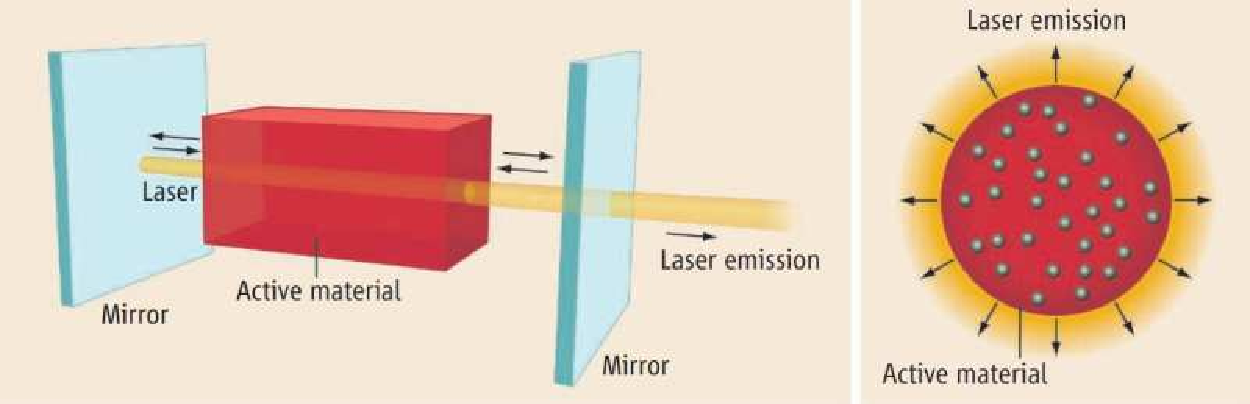
\includegraphics[width=12cm]{./Figs/F1_medium}
\end{center}
\caption[Unified models for light emitting in optical cavities.]{\textbf{Two models for light emitting in optical cavities.} (Left) Sketch of a conventional Fabry-Perot (F-P) laser cavity model: Light is tightly confined by a cavity with a given geometry shape that defines the resonant cavity modes and laser frequency. (Right) A random laser cavity model: Light is scattered by a set of photon emitting particles which modify the optical properties of the optical cavity. This thesis discusses the modification effect of emitters ensemble to the optical cavities in the linear optical regime. From~\cite{Bravo-Abad2008}. Reprinted with permission from AAAS.}
\label{unifiedlasermodel}
\end{figure}



%This work is an extension of previous success on a few excitons coupled cavities studies using scattering model~\cite{Yao2009b,Yao2009c,Yao2009a,VanVlack2011,Reitzenstein2010,Hughes2009,Kristensen2011}. %But for GF calculations involving a large amount of emitters, present works are only limited to a few cases, either within a very narrow frequency range~\cite{Averkiev2009} or ignoring iterated interactions between emitters~\cite{VanVlack2011}, because fully calculation using GF method is a memory- and CPU-time-costly work. This paper will report the spectral modification effects of up-to thousands of emitters for coupled cavities in a broad frequency range and with fully scattering interactions.

%Beyond the motivation in physics mentioned above, there is also a personal motivation strongly driving me to answer some sophisticated questions in the course of researching in theoretical physics. Not too long since I began to study at Queen's University, something really shocking happened to me. Issues arose with my previous supervisor around difference concerning basic principles, which I believe should not be given up. I was thinking about the meaning of life, the driving power of this world, and how I can survive this crisis. The world became both ugly and elegant, cold and warm, bitter and sweet, noisy and melodic, detached and crowded, greedy and generous, selfish and altruistic, impartial and fair... I came to a place of acceptance and decided to finish up the scientific research following my own line of inquiry. Collective interaction in nature may offer insight into the secrets I expect to explore and be significant to this world on many levels. This thinking and reflecting has led to the motivations and problems partially reflected in the scientific side of this thesis.
\section{Background}
In this section, to provide background, we present an overview of optical cavities, photon emitters and present commonly used photonic simulation methods.

\subsection{Optical Cavities}
An optical cavity is a structure that can confine the light in a limited space called cavity, and creates a relatively strong optical field to enhance light-matter interactions. A typical optical cavity is formed by arranging a set of ``mirrors'' or reflecting surfaces in a certain pattern so that the light is reciprocally reflected between them, and the optical fields of different light paths are superimposed to give a strong optical field in the cavity. The most simple pattern of mirror arrangement gives a cavity called Fabry-Perot (F-P) cavity, which has two plane mirrors in parallel to each other (see Fig.~\ref{unifiedlasermodel} left).

The reflectivity of the mirrors, which is defined as the ratio of the power of the reflected light to that of the incident light, determines how many times the light can travel in between the mirrors before decayed leaking out of the cavity. If a cavity is to induce strong interactions between light and the matter in the cavity, the cavity field must be strong enough, compared to the field strength around an electron without the cavity environment. It is necessary to increase the reflectivity of the mirrors in order to enhance the light-matter interactions in the cavity. The highest reflectivity is $100\%$; however, it is unnecessary to make it so high, because we usually need some output from the cavity for other purposes such as lasing. Once the reflectivity is not $100\%$, there is loss or dissipation in a cavity. The ratio of the energy stored to the lost in a cavity is called the Q-factor, denoted by $Q$. Obviously, the higher is the Q, the stronger the cavity field. A typical $Q$ value for a useful optical cavity ranges from several thousands to $10^8$~\cite{Vahala2003}.

The light confined by a cavity has to be essentially a standing wave, otherwise, it will be weakened and canceled by the many superpositions in the cavity~\cite{Novotny2006}. In this sense, an optical cavity is also called an optical resonator. Actually, lasers are typical applications of optical cavities, due to the frequency selection function of cavities. There are certain frequencies that survive, in which the light can permitted to propagate in a cavity. Each frequency corresponds to one mode or more. A mode is defined as a field distribution pattern for a given cavity at a certain frequency. The mode is mainly determined by the geometry of the cavity. The mode volume, $V_{eff}$, describes the concentration of normalized field strength considering the distribution of the refractive index of the cavity medium. It has a unit of volume. If the cavity field is well confined in a small region, the photon emitter in this region can be strongly coupled to the cavity field and show some non-classical or quantum behaviors. The coupling strength, $g\propto 1/\sqrt{V_{eff}}$, describes how strongly a photon emitter is coupled to the cavity field and is forced to emit or absorb photons under the influence of the cavity.  The smaller the mode volume is, the more the cavity field concentrates, and the more clearly the quantum behaviors are observed. To be specific, in this thesis we mainly focus on microcavities, which have typical mode volumes smaller than $10^3\,\mu m^3$. Some microcavities can emit single photon in each emission pulse~\cite{Schwagmann2011,Yao2009a}.

The $Q$ factor can be also defined as the confinement time in units of optical period, such that $Q=\frac{2\pi\tau}{T}=\frac{\omega_c}{\Gamma_c}$, where $\tau$ is the average lifetime of a photon in the cavity, $T$ is the optical period of a given cavity mode, $\omega_c$ is the mode's angular frequency, and $\Gamma_c=1/\tau$ is the decay rate of the cavity. In the presence of cavity decay, the cavity spectrum has a bandwidth, spectral width or linewidth characterized by $\Gamma_c$. The study of this thesis mainly focuses on how the cavity resonance, $\omega_c$, and decay rate or spectral width, $\Gamma_c$, are changed, with the coupling of many photon emitters. By understanding the mechanism of emitter-cavity interactions, one can design and fabricate novel photonic devices for optical communication, quantum computing and many other applications. Before stepping into light-matter interaction, we introduce some typical microcavities.

Microcavities have different structures.  The ones of interest in this thesis are realized in semiconductors which are good materials to form photon emitters included in a cavity. The cleavage planes of semiconductor crystals can be used as the mirrors for a F-P cavity. However, the reflectivity of a cleavage plane is too small to form a high-Q cavity. A distributed Bragg reflector (DBR), which is formed from multiple layers of alternating materials with varying refractive index, is usually used to enhance the Q-factor of a F-P type cavity. A micropillar laser~\cite{Vahala2003} is formed by using DBRs in 1-dimention (1-D). To further increase the Q-factor, 2- and 3-D confinements of light are helpful. A whispering-gallery-type cavity is a 2- or 3-D confined cavity, in which the light is reflected around the circular or spherical wall through total internal reflection.

A photonic crystal (PC) cavity is another type of high dimensional confined cavity. A PC is a photonic structure which has periodic variation of refractive index in 1-D, 2-D or 3-D space. The periodic structure creates a certain frequency band called photonic forbidden band or band gap (PBG), so that a light in this band cannot propagate. By adding a ``defect'' in the PC structure, a permitted narrow band is formed in a certain direction so that a light in this small frequency range is allowed to emit out of the cavity in a certain direction while reflected in the other directions through total internal reflection. The periodic arrangement of refractive index forms the photonic lattice. A ``defect'' in a PC structure is a break region of the periodical structure to form a cavity. It implies that a PC cavity is a photonic structure with periodic variation of refractive index and with a defect. The micropillar laser is a 1-D PC cavity.

The 2-D PC cavity studied in this thesis is called the H3 PC cavity. It is formed from a thin slab of material with a triangular lattice with three neighboring holes (usually airholes) removed in a line to form the cavity (see Fig.~\ref{FDTDsimulation}). A triangular lattice is a pattern of holes arrangement that every three nearest holes are on the vertexes of a equilateral triangle, where the side length of the triangle is the lattice period or pitch. The H3 PC cavity provides a large PBG for TE-like light in the slab made by InP, GaAs or silicon~\cite{Johnson2002a}. With a given material of slab, the resonance of the cavity can be tuned by changing the pitch, the radius of the holes or the distance between the airholes at the ends of the cavity. The uniformity of the hole sizes and positions, the roughness of fabrication, and the distance between the airholes at the ends of the cavity affect the decay rate of the cavity~\cite{Akahane2003}. The silicon-based H3 PC cavity used in this thesis is set to have the following parameters: the lattice period $a=420$ nm, the radius of the holes $r=115.5$ nm, the distance between the holes at the ends of the cavity is $1806$nm, and the thickness of the slab is $210$ nm. The finite difference time domain (FDTD) simulation (will be introduced shortly) gives the resonance of $191.551$ THz, the effective mode volume of $\sim 0.07\,\mu m^3$ and $Q$ is above $45,000$. The refractive index of the slab used in our FDTD simulation is $3.46$. We do not use the Q-factor and the decay rate obtained from FDTD simulation in our exciton-cavity interaction analysis, rather we numerically set the decay rate and Q-factor to match with published studies. According to the relationship of $Q=\frac{\omega_c}{\Gamma_c}$, therefore, the cavity resonance may be different from the FDTD simulation result. In most cases, we set $\Gamma_c=0.1$ meV, which gives $Q\approx 8000$.

\begin{figure}[htp]%[floatfix]
\centering
\begin{center}
%\DeclareGraphicsRule{.pdf}{eps}{}{`convert #1 eps:-}
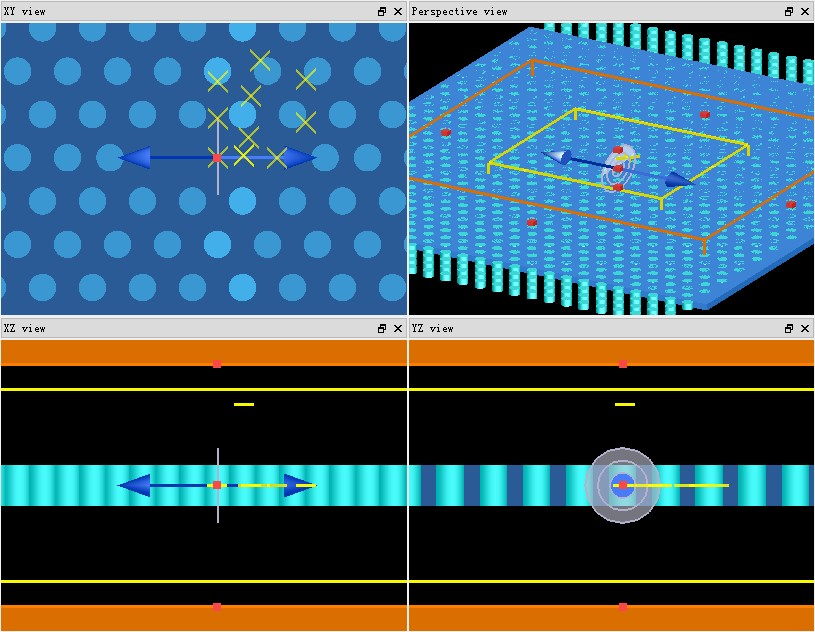
\includegraphics[width=10cm]{./Figs/FDTDsimulation}%[bb=1.0in 1.0in 7.5in 10in]
\end{center}
\caption[An FDTD simulation diagram of a H3 PC cavity.]{\textbf{An FDTD simulation diagram of a H3 PC cavity.} Top right shows the 3-D bird-view of the cavity configuration under simulation. Top left shows the zoomed-in top-view on the cavity, where three airholes (in light blue) are removed from the triangle lattice. Bottom left shows the $x$-$z$ view. Bottom right shows the $y$-$z$ view. Double arrows indicate a dipole source is in the center of the cavity. Cross signs indicate the in-site time monitors in an FDTD simulation.}
\label{FDTDsimulation}
\end{figure}


A PC cavity structure can be fabricated using epitaxial growth technique and standard semiconductor planar processing technology. The slab can be grown layer by layer using metalorganic vapor phase epitaxy (MOCVD) or molecular beam epitaxy (MBE) technologies in the scale of $0.1$ nm or so~\cite{III2009}. The components and growth conditions can be monitored and tuned in real-time to control the growth quality. Quantum wells and quantum dot layers can be formed by tuning growth conditions such as temperature, pressure, flow rate or supplying rate and so on. After the slab is grown, photolithography technology can be used to form the pattern of the hole arrangement. Some type of photoresist and a patterned mask are used in the photolithography process, and the pattern in the mask is transformed to the photoresist layer on top of the slab. Some parts of the photoresist layer are removed under $X$-ray exposure in the process. By using wet etching or dry etching technologies, the pattern is consequently transformed to the arrangement of holes by vertically etching off the materials of the slab uncovered by photoresist.


\subsection{Quantum Dots and Optical Emitters}
A cavity without photon emitters is useless unless the cavity is used as a pure coupler to an incident light. Photon emitters in a cavity can generate absorption and gain so that a laser or a light beam with a certain property is emitted from the cavity, and make the cavity functional. In this thesis, we only consider quantum photon emitters, which emit light mainly through quantum transitions or quantum jumps rather than thermal radiations. Some types of atoms, ions and electron-hole pairs in a certain environment can be the units of such quantum photon emitters, which emit photon through the transition of electrons in them from a high level to a low level, or through annihilation of electron-hole pairs (will be introduced in Chapter~\ref{ch:theory}). A nitrogen vacancy, a quantum well or a quantum dot (QD) provides the necessary environment for quantum transitions. Because of good thermal characteristics and excellent optical and electronic performances, QDs are widely used. We will use QDs as an example of quantum emitters in our discussion.

%Electrical and optical pumps are two ways to excite the emitters. In this thesis, we only interest in optical pump case, in which a pumping light is emitted to the cavity; the emitters absorb the light and re-emit the light with the interaction of the cavity. The emitted light usually has different properties such as frequency and bandwidth from the incident light. The differences and the mechanism is the study topic in this thesis.

In a simple model, a QD can be treated as a 0-D or 3-D quantum box, which confines electrons in a small condensed space. The electrons in a QD have discrete energy levels because of the quantum confinements from the nearby interface atoms. The energy discretization makes the quantum transition of states possible to emit photons. In practice, a QD is usually made of semiconductor materials such as InGaAs/GaAs, AlGaAs/GaAs and Ge/Si. As mentioned earlier, QDs can be grown through epitaxial growth technique~\cite{Schliwa2009}, which grows semiconductor materials layer by layer. Through changing the growth conditions, dot-shape bumps can be formed. Those bumps are quantum dots. We call the QDs grown in this method as self-assembled QDs, which are randomly distributed in a layer. QDs can also be grown through Hydrothermal method and sol-gel growth method, in forms of random nanocrystals. Self-assembled QDs usually have a dimension of $5\sim 150$ nm, a intrinsic decay rate ranging from several to several tens of $\mu$eV, and a density of $10^{10}\sim 10^{11}$/cm$^2$~\cite{Amano2006}. The size of a QD affects its emission resonance or frequency; the quality of growth and the slab environment affect its decay dynamics. Typically, there can be more than thousands of self-assembled QDs in an effective interaction area $\sim \mu m^2$, and the QD resonances are distributed in a Gaussian (normal) distribution profile or a logarithmic normal distribution profile with a standard deviation ranging from several to several tens of meV. We will discuss a cavity with {\textit {discrete}} and {\textit {dense}} QDs in later chapters, where there are several tens and several thousands of quantum emitters respectively.

\subsection{Simulation Methods}
One can simulate the mode distribution and calculate the mode resonance of a cavity using numerical methods. The finite element method (FEM) and finite-different time-domain (FDTD) method~\cite{Taflove2005} are two mature methods for the cavity analysis. The idea is to solve the Maxwell equations of the optical field with boundary conditions determined by the cavity geometry. The FDTD method solves the differential equations in the time domain and through meshing the geometric structure into small unit Yee cells~\cite{Taflove2005}. The FEM solves the corresponding integral form of Maxwell equations with finite Discretization of the cavity geometry structure based on Gauss-Green theorem. Packaged softwares such as PICS3D, COMSOL Multiphysics, R-Soft suit, Lumerical FDTD Solutions and Meep have been developed based on these two methods. We use Lumerical FDTD Solutions~\cite{LumericalSolutions} to simulate the bare cavity properties.

To calculate the cavity mode in FDTD solutions, one has to put a light source into the cavity to generate a propagating optical field in the time domain (see Fig.~\ref{FDTDsimulation}). We use a dipole source as the light source. Note that the dipole sources used in FDTD simulation is not the dipoles studied in this thesis for exciton-cavity interactions. The dipole sources in FDTD simulation can generate a light field as a dot light source under predefined parameters, but it does not interact with the cavity, which means the dipole source's properties cannot be changed by the optical field, and the dipole source cannot scatter light traveling toward it. In fact, there is no mature software which can fully simulate the complex cavity interactions with many photon emitters. This is why we conduct the study present in this thesis.


In our study, at first, we calculate the bare cavity mode without photon emitters using FDTD method; then we include the photon emitters into the cavity system based on Green function (GF) method (will be introduced in the next chapter), in which every photon emitter is treated as a dipole. We will discuss the cases that one- and two-dipole coupled to a cavity, discrete-dipole coupled to a cavity and dense-dipole coupled to a cavity to study the exciton ensemble-cavity or ensemble-cavity interactions in detail. The density of dipole distribution referred in this thesis is mainly used as a concept of describing how close the dipole resonances to each other in the frequency domain rather than in the spatial domain.

\section{Problems}
There are four major questions that I wish to address on the topic of exciton-cavity interactions:

a) How does an ensemble of emitters affect the optical properties of a cavity with which the emitters are coupling?

b) How does a cavity affect an ensemble of individual emitters that are coupling to it? Can we explain the spectral behaviors by considering the collective emitting and light scattering process?

c) Can we always view a photon emitting unit, for example, a QD, as one single exciton? How do optical pumps excite excitons?

d) Upon the excitation of emitters, can the cavity mode and the coupling condition of excitons be changed?


This thesis undertakes to answer these four questions rigorously and scientifically.

%If, for example, one replaces ''emitters'' with ``people'', or replaces ``cavities'' with ''communities''  in the questions above, one may see an aspect of the questions I was concerning myself with the social side. However, in what follows, we will confine our discussion to the interaction of emitters and cavities problems.

Technically, to fully understand the physics of cavity-emitter interaction, we need to calculate every interaction path between cavity and individual emitters. How to calculate the cavity spectrum considering these interaction channels is another problem in our study, which ultimately leads to an open work on making a nanophotonic toolbox to make calculation processing efficient.

\section{Objective}
In this thesis, we calculate the optical parameters of a photonic crystal (PC) H3 cavity (mainly) using the finite-different time-domain (FDTD) method and  calculate the ensemble spectrum of a few QDs in a PC cavity. Then, we develop a method to calculate a dense-emitter-coupling cavity spectrum. Through these calculations and comparing the results with that of simplified models, we answer the four problems referred to above (see Fig.~\ref{Cavity_pump}).

%    \notesbox{Note:  These are the section headings that I decided to use.  Check out several
%    recent theses to decide how you want to lay out your introduction (and conclusion) chapters.}

\begin{figure}[htp]%[floatfix]
\centering
\begin{center}
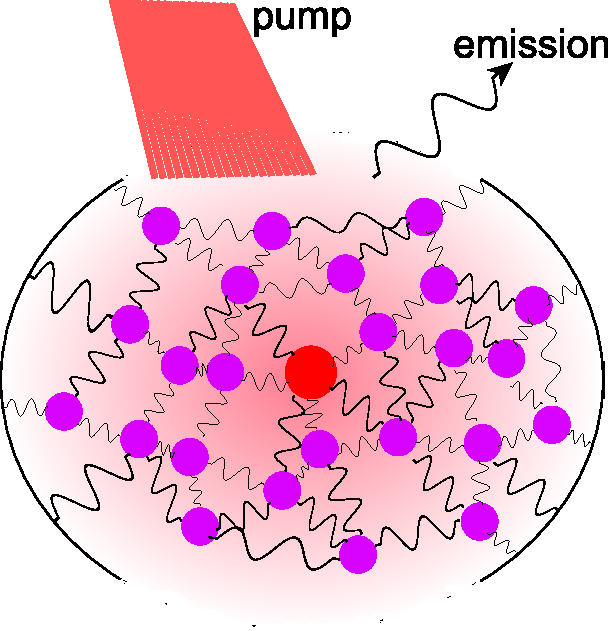
\includegraphics[width=6cm]{./Figs/Cavity_pump}%[bb=1.0in 1.0in 7.5in 10in]
\end{center}
\caption[Many photon emitters are coupled to a cavity.]{\textbf{Many photon emitters are coupled to a cavity.} In the linear optics regime, this thesis will study the changes of the cavity properties, the mechanism of optical pumps and the role of background emitters (purple balls in the figure) to the cavity, a target emitter and their coupling. The red ball at the center of the cavity indicates the target dipole which is on resonance and in a strong field.}
\label{Cavity_pump}
\end{figure}

\section{Hypothesis}
This thesis focuses on the light-matter interaction in a ``general`` schema while also including hypotheses that make our discussion less ``general``. For example, this study always uses the dipole approximation, which means that every exciton excited in photon emitters can be treated as a dipole. Notice that there is no strong correlation between the number of physical emitters, such as QDs, and that of dipoles we are using for our discussion. This assumption is commonly acceptable in the cases in which the electromagnetic field can be viewed as a constant homogeneous field on the scale of an emitter, which is valid for QDs and color centers in normal nanocavities. However, this assumption also means we do not consider the band structure of the emission units; rather, we mainly focus on the emitting and scattering nature of individual emitters merged in a dielectric environment. Hence, our work cannot explain the intraband absorption of QDs, Auger recombination, spin splitting, and other phenomena which involve complex band structures.

For the calculation based on the FDTD method and our Green function (GF) method, we assume that the cavity mode can be described by Maxwell equations, which is usually valid for normal nanophotonic devices, including all the cavity configurations we are going to discuss in this thesis.

For the calculation based on the GF method, we also always use the single excitation approximation~\footnote{There is only one exciton or photon in the cavity.} and only consider the linear effect of dipole-dipole and dipole-cavity interactions, which may not work for high-power pumped cavities or explain the spatial hole burning effect, but is good enough to reveal the physics of ensemble-cavity interaction in our scenarios.




\section{Organization of Thesis}

We begin the thesis by introducing necessary background, including photonic scattering theory and the Green function method, the initial condition of my calculations, as well as the statistical method of master equations in
chapter~\ref{ch:theory}. We discuss typical photonic nanocavities mode calculations with the FDTD method and Green function calculation algorithms, and study the spectrum and GFTs of cavities with a few discrete dipoles in Chapter~\ref{ch:cavity}. The methods and models we used in this thesis will be verified in this chapter. It will also identify the effects of modifying the optical property of a cavity and dipoles. Chapter~\ref{ch:ensemble} describes our work on the spectrum of cavities coupled with a dense quantity of photon emitters using the GF method, compared with master equation (ME) models, for several scenarios of random dipole distributions. Spectral modification effects will be studied in the presence of dense dipoles.
Chapter~\ref{ch:Conclusion} concludes the findings of this study, and outlines the future work. The overall structure of my research is shown in Fig.~\ref{MainStructure}.
Implementation details and long derivations of the calculations, calculation methods and some key formulas are presented in the appendices.

\begin{figure}[htp]%[floatfix]
\centering
\begin{center}
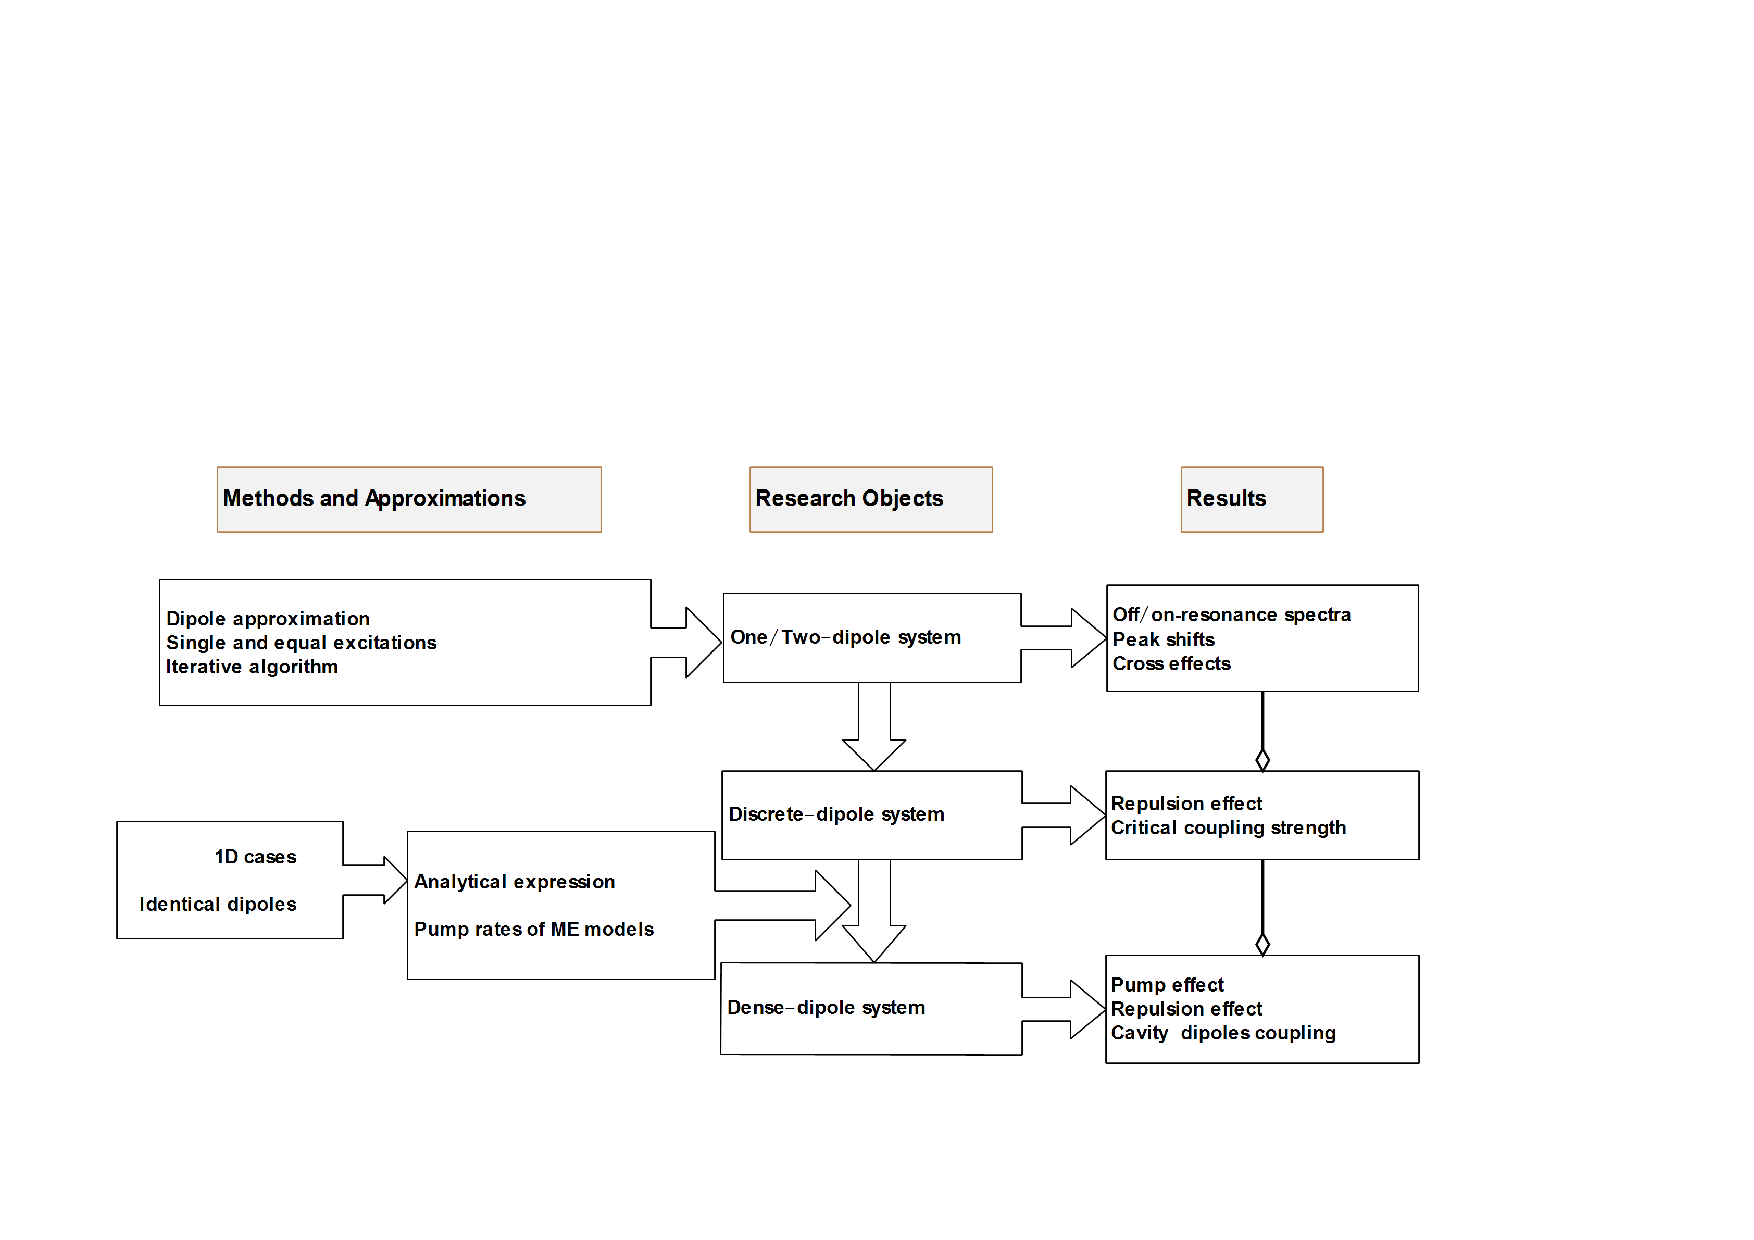
\includegraphics[width=16cm]{./Figs/MainStructure}%[bb=1.0in 1.0in 7.5in 10in]
\end{center}
\caption[Hypotheses, research objects and main results.]{\textbf{Hypotheses, research objects and main results.} }
\label{MainStructure}
\end{figure} 